
\documentclass[final,hyperref={pdfpagelabels=false},16pt]{beamer}
\usetheme{Berlin}
\usefonttheme{professionalfonts} % using non standard fonts for beamer
\usefonttheme{serif} % default family is serif

\usepackage[russian]{babel}
\usepackage[utf8]{inputenc}
\usepackage[orientation=portrait,size=a0,scale=1,debug]{beamerposter}
\usepackage
	{
		% Дополнения Американского математического общества (AMS)
		amssymb,
		amsfonts,
		amsmath,
		amsthm,
		physics,
		graphicx
		}
\setbeamertemplate{navigation symbols}{} % минус навигация
\setbeamercolor{block body}{bg=white}
\setbeamerfont{block title}{series=\bfseries}
\let\Tiny=\tiny % решает проблему со шрифтами в TexLive
\setbeamertemplate{headline}{
	\leavevmode
	\begin{beamercolorbox}[wd=\paperwidth]{headline}
		\vspace{2ex}\\
		\begin{columns}[c]
			\begin{column}{.09\paperwidth}
			\end{column}
			\begin{column}{.675\paperwidth}
				\raggedleft
				\usebeamercolor{title in headline}{\textbf{\Huge{\inserttitle}}\\[1ex]}
				\usebeamercolor{author in headline}{\large{\insertauthor}\\[1ex]}
				\usebeamercolor{institute in headline}{\small{\insertinstitute}\\[1ex]}
			\end{column}
			\begin{column}{.25\paperwidth}
				\begin{center}
                    \begin{minipage}{0.49\linewidth}
                        
\includegraphics[width=\textwidth, keepaspectratio]{rf3}
                        
                    \end{minipage}
                    \begin{minipage}{0.49\linewidth}
                        
\includegraphics[width=\textwidth, keepaspectratio]{iap}
                        
                    \end{minipage}

                    \hfill
				\end{center}
			\end{column}
			\begin{column}{.03\paperwidth}
			\end{column}
		\end{columns}
		\vspace{2ex}\\
	\end{beamercolorbox}

 	\begin{beamercolorbox}[wd=\paperwidth]{lower separation line head}
		\rule{0pt}{2pt}
	\end{beamercolorbox}
	\vskip-2cm
	}

\setbeamertemplate{footline}{
	\begin{beamercolorbox}[wd=\paperwidth]{upper separation line foot}
		\rule{0pt}{2pt}
	\end{beamercolorbox}
	\leavevmode%
	\begin{beamercolorbox}[ht=4ex,leftskip=1cm,rightskip=1cm]{author in head/foot}%
		{Оформлено при помощи издательской системы \LaTeX}
        \hfill
		\today
		\hfill
        Github: {github.com/kannab98},   Email: {ponur0kirill@gmail.com}
		\vskip1ex
	\end{beamercolorbox}
	\vskip0pt%
	\begin{beamercolorbox}[wd=\paperwidth]{lower separation line foot}
		\rule{0pt}{2pt}
	\end{beamercolorbox}
	}

\title{Численное моделирование морской поверхности}
\author{Понур К.А.$^{1}$, Караев В.Ю.$^2$, Рябкова М.С.$^2$}
\institute{$^{1}$ Нижегородский Государственный Университет им. М.Ю. Лобачевского \\
          $^2$ Институт Прикладной Физики Российской Академии Наук}
\date{\today}
\newcommand{\tK}{\widetilde{K}}
\usepackage{mathtools}
\mathtoolsset{showonlyrefs}
\newcommand{\mean}[1]{\langle #1 \rangle}
\begin{document}
  \begin{frame}[t]{} 
    \begin{columns}[t]
      \begin{column}{.48\linewidth}
        \begin{block}{Введение}
            Сегодня активно изучается процесс взаимодействия излучения больших мощностей с плазмой. На данный момент в экспериментах с использованием фемтосекундных лазеров удалось получить импульсы интенсивностью до $10^{22}$ Вт/см$^2$. В случае взаимодействия столь мощного излучения с плазмой возможно образование особых лазерно-плазменных структур. Изучение подобных структур представляет собой фундаментальную задачу и имеет ряд практически важных применений. Ускорение ионов $-$ одно из них. 

            В данной работе исследуются структуры, образующиеся при падении мощного лазерного излучения на бесконечно толстую мишень в режиме ускорения ионов, который известен как режим «плуга».
        \end{block}


        \begin{block}{Модель}
           % На полубесконечную непрозрачную плазму падает перпендикулярно циркулярно поляризованное излучение большой интенсивности. 

            В построенной модели используется ряд приближений. 
            \begin{enumerate}
            \item циркулярно поляризованное излучение
            \item полубесконечная непрозрачная плазма
            \item случай "холодной" плазмы
            \item движения одномерные в отсутствии поперечных неустойчивостей
            \item задача решается в движущейся система отсчета, связанной с точкой разворота плазмы (b)
            \item используется приближение четырехжидкостной гидродинамики - движение частиц представимо в виде движения электронных и ионных потоков
       
 			\end{enumerate}
        
        \begin{figure}[h]
            \begin{minipage}{0.47\linewidth}
                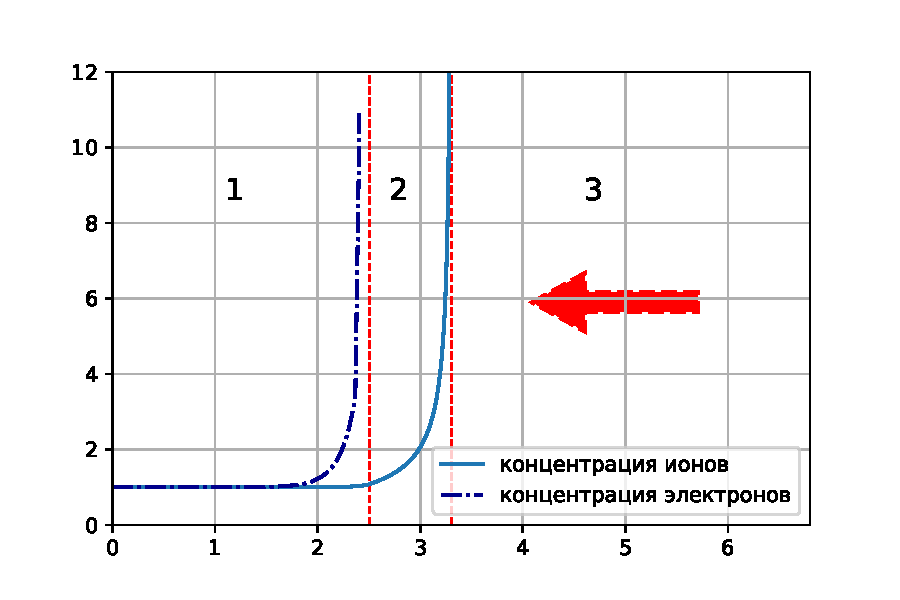
\includegraphics[width=\linewidth]{pic/1jstruct.pdf}
                \centering
                (a)
            \end{minipage}
            \begin{minipage}{0.47\linewidth}
                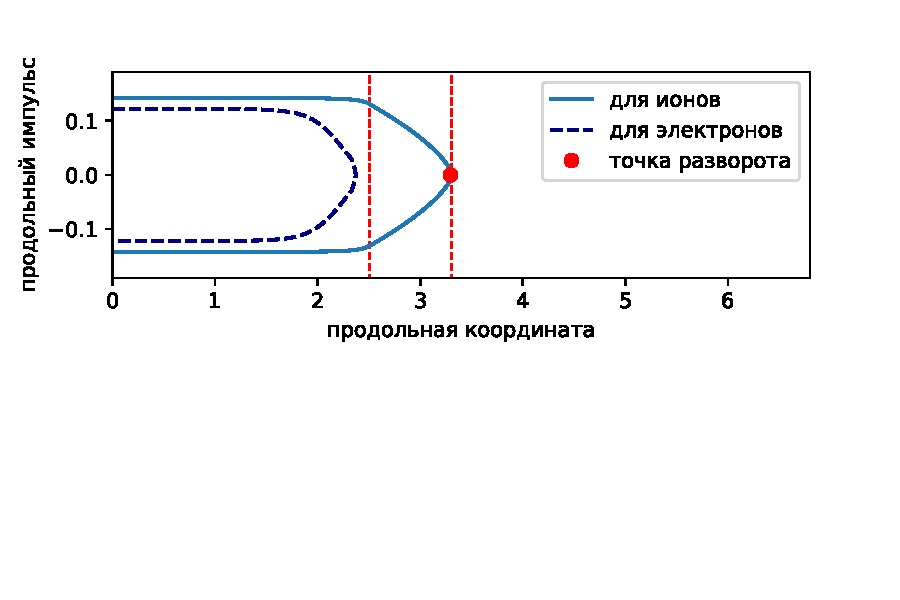
\includegraphics[width=\linewidth]{pic/2jstruct.pdf}
                \centering
                (b)
            \end{minipage}
            
            \label{fig:spec}
            \caption{Ускоряющая стуктура плазменного слоя в режиме плуга. В задаче присутствуют три области: вакуумная(3), ионная(2) и плазменная(1). }
        \end{figure} 


        	%Задача решается в движущейся система отсчета, связанной с точкой разворота плазмы. 
        	%Используется приближение четырехжидкостной гидродинамики - движение частиц представимо в виде движения электронных и ионных потоков.
        \end{block}

        \begin{block}{Система уравнений и картина решений}
            Поведение волны удобно описывать в терминах векторного и скалярного потенциалов электромагнитного поля. 
            Исходные уравнения имеют вид:

$$\dv[2]{\varphi}{z}=4\pi e(N_e-Z_iN_i)$$
%Здесь $N_e$-концентрация электронов, $N_i$-концентрация ионов, $Z_i$-степень ионизации ионов (равная для всех ионов).

$$\Delta \vec A-{{1}\over{c^2}}\pdv [2]{\vec A}{t}={{1}\over{c}}\pdv{\nabla \varphi}{t}+{{4\pi}\over{c}}(eN_e \vec v_e-eN_iZ_i\vec v_i)$$

\vspace{1.2em}

Здесь $N_e$-концентрация электронов, $N_i$-концентрация ионов, $Z_i$-степень ионизации ионов (равная для всех ионов).
%Рассматриваем стационарный случай, тогда в проекциях на z и перпендикулярную плоскость получим:
Рассматривается случая монохроматического и циркулярно поляризованного поля:
\vspace{1.2em}
$$\vec A_\perp(z,t)=Re\{A(z)(\vec x_0+i\vec y_0)e^{i\omega t}\}$$
Вводя безразмерные переменные 

\begin{gather}
  \widetilde\varphi={{e\varphi}\over{m_ec^2}}, \quad
  \xi={{\omega z}\over{c}}, \\
  n_e={{N_e}\over{N_e^{\infty}}}, \quad
  n_i={{N_i}\over{N_i^{\infty}}}={{N_iZ_i}\over{N_e^{\infty}}}
\end{gather}

$$a={{eA}\over{m_ec^2}}$$
%и учитывая факт нейтральности плазмы на бесконечности: $Z_iN_i^{\infty}=N_e^{\infty}$, получим: 
%$$\dv[2]{\widetilde \varphi}{\xi}=n_0(n_e-n_i)$$

%где введен параметр $n_0={{4\pi e^2 N_e^{\infty}}\over{m_e\omega^2}}$

%$$\Delta \vec A-{{1}\over{c^2}}\pdv [2]{\vec A}{t}={{1}\over{c}}\pdv{\nabla \varphi}{t}+{{4\pi}\over{c}}(eN_e \vec v_e-eN_iZ_i\vec v_i)$$
%Рассматриваем стационарный случай, тогда в проекциях на z и перпендикулярную плоскость получим:
%$$\dv[2]{a}{\xi}+(1-{{n_0n_e}\over{\gamma_e}}-{{n_0n_i}\over{\gamma_i}}\mu)a=0$$
%В силу малости $\mu$ пренебрежем последним слагаемым.
\vspace{1.2em}

		 Для описания движения электронной и ионной компонент обратимся к уравнениям гидродинамики:

$$\pdv{\vec p_e}{t}+(\vec v_e \nabla)\vec p_e={{e}\over{c}}\pdv{\vec A}{t}+e\nabla\varphi-{{e}\over{c}}[\vec v,rot\vec A]$$
$$\pdv{\vec p_i}{t}+(\vec v_i \nabla)\vec p_i={{eZ_i}\over{c}}\pdv{\vec A}{t}-eZ_i\nabla\varphi-{{eZ_i}\over{c}}[\vec v_i,rot\vec A]$$
%Тогда в безразмерных переменных получаем:
%$$\dv{\widetilde \varphi}{\xi}=\dv{\gamma_e}{\xi}$$
%$$-\dv{\widetilde \varphi}{\xi}={{m_i}\over{Z_im_e}}\dv{\gamma_i}{\xi}$$
\vspace{1em}

Вводим обозначения: $\mu=Z_i{{m_e}\over{m_i}}<<1$, $\widetilde p_e={{p_{ez}\over{m_ec}}}$, $\widetilde p_i={{p_{iz}\over{m_ic}}}$

%\vspace{0.7em}
\begin{equation}
        	       \begin{cases}
            \varphi''=n_0(n_e-n_i)\\
            a''+(1-{{n_0n_e}\over{\gamma_e}})a=0\\
             \varphi=\sqrt{1+a^2+\widetilde p_e^2}-\sqrt{1+\widetilde p_e^{\infty2}}\\
            -\varphi={{1}\over{\mu}}(\sqrt{1+a^2\mu^2+\widetilde p_i^2}-\sqrt{1+\widetilde p_i^{\infty2}})
            \end{cases}
        \end{equation}

\vspace{1em}
Для её решения необходимо учесть условия на бесконечности:
%\vspace{0.8em}

\begin{gather}
  n_e\widetilde v_e=\beta^\infty, \quad 
  n_i\widetilde v_i=\beta^\infty, \\
  \widetilde p_e=\gamma_e \widetilde v_e, \quad
  \widetilde p_i=\gamma_i \widetilde v_i
\end{gather}
%$$\widetilde p_i=\widetilde v_i\sqrt{1+\widetilde p_i^2}$$
%$$\widetilde p_i^2={{\beta^{\infty2}}\over{n_i^2-\beta^{\infty2}}}$$
%$$\widetilde p_e^2={{\beta^{\infty2}(1+a^2)}\over{n_e^2-\beta^{\infty2}}}$$
%$$(-\varphi\mu+\gamma_i^\infty)^2=1+{{\beta^{\infty2}}\over{n_i^2-\beta^{\infty2}}}={{n_i^2}\over{n_i^2-\beta^{\infty2}}}$$
%$$n_i^2={{\beta^{\infty2}(-\varphi\mu+\gamma_i^\infty)^2}\over{(-\varphi\mu+\gamma_i^\infty)^2-1}}$$
%$$(\varphi+\gamma_e^\infty)^2=1+a^2+{{\beta^{\infty2}(1+a^2)}\over{n_e^2-\beta^{\infty2}}}={(1+a^2){n_e^2}\over{n_e^2-\beta^{\infty2}}}$$
%$$n_e^2={{\beta^{\infty2}(\varphi+\gamma_e^\infty)^2}\over{(\varphi\mu+\gamma_e^\infty)^2-a^2-1}}$$
\vspace{0.6em}

  Окончательная система уравнений имеет вид:
\begin{equation}
\begin{cases}
    \varphi''(z)=n_0\beta^{\infty}\left({{\varphi+\gamma_e^{\infty}}\over{\sqrt{{{(\varphi+\gamma_e^{\infty})^2-a^2-1}}}}}-{{\gamma_i^{\infty}-\varphi\mu}\over{\sqrt{(\gamma_i^{\infty}-\varphi\mu)^2-1}}}\right) \\
    a''(z)=-a+{{n_0\beta^{\infty}}\over{\sqrt{(\varphi+\gamma_e^{\infty})^2-a^2-1}}}a \\
\end{cases}
\end{equation}

        \begin{figure}[h]
            \begin{minipage}{0.5\linewidth}

                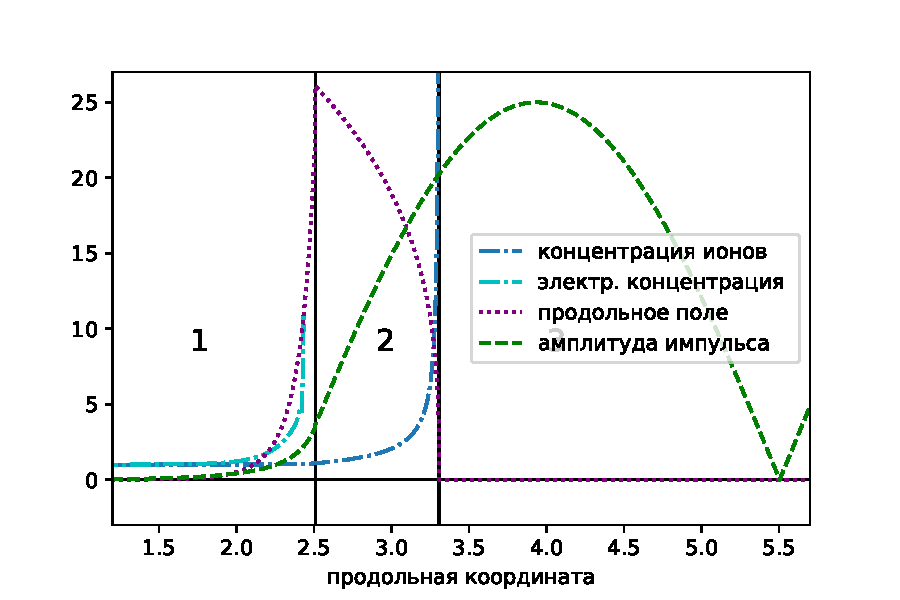
\includegraphics[width=\linewidth]{pic/3jstruct.pdf}
                %\centering
                
            \end{minipage}
            
            \caption{Структура решений при ускорении ионов в режиме "плуга" (штриховой линии соответствует модуль комплексной амплитуды лазерного поля, пунктиром показана структура продольного электростатического поля, штрих-пунктирной линии соответствуют концентрации электронов и ионов)}
        \end{figure}

        
      
            


        \end{block}
        
  	\end{column}
      \begin{column}{.48\linewidth}

        \begin{block}{Учет продольной температуры электронов}
            При относительно небольших температурах ее влияние можно оценить в рамках анализа движения пробных электронов, имеющих скорость отличную от средней гидродинамической. Такой анализ удобно проводить путем построения фазового портрета. 

            Гамильтониан движения электрона имеет вид:

            \begin{equation}
                H(z,p_z)=\gamma(z,p_z)-\varphi(z)
            \end{equation}

            \vspace{0.6em}
            Тогда уравнения движения электрона записываются в виде:

                \begin{center}
                    \begin{equation}
                    \begin{cases}
                    	\dot z={{p_z}\over{\gamma}} \\
                    	\dot p_z=-\frac{\partial\gamma}{\partial z}-E_z(z) \\

                    \end{cases}  
                    \end{equation}
                    \vspace{0.6em}
                    где $\gamma(z,p_z)=\sqrt{1+a^2(z)+p_z^2}$
                \end{center}
\vspace{0.6em}
                 На границе плазма -- ионный слой существует состояние равновесия типа центр. На фазовом портрете также существует седло (S), сепаратрисы, которого разделяют потоки траекторий частиц, уходящих в вакуум и возвращающихся в плазму. В вакуумной области состояния равновесия центр и седло чередуются, что соответствует стоячей волне.
                
                Значение критического импульса электрона на границе плазмы будет соответствовать значению сепаратрисы седла S в граничной точке. 

                \begin{equation}
                	p_z=0, {{a}\over{\sqrt{1+a^2(z)}}}\frac{\partial a}{\partial z}+\frac{\partial\varphi}{\partial z}=0
                \end{equation}
\vspace{0.6em}
                \begin{equation}
                	H_{cr}=H(z_b,0), p_{cr}=\sqrt{(H_{cr}+\varphi(z_s))^2-a^2(z_s)-1}
                \end{equation}

\vspace{0.6em}
                Если электрон обладает импульсом, который больше критического, он покидает границу. Если таких электронов достаточно много, то устойчивость структуры нарушится. Таким образом можно оценить температуру, при которой происходит разрушение стационарного режима ускорения ионов в режиме «плуга».
                Фазовый портрет такого вида получается не при любых соотношениях параметров задачи. Входными параметрами являются параметр закритичности плазмы и амплитуда падающей волны. При некотором изменении параметров волна перестает полностью отражаться, что на фазовом портрете соответствует исчезновению ограниченных траекторий в вакуумной области. Таким образом, существует порог , выше которого существует режим «плуга», ниже – излучение проходит в плазму.

                \begin{figure}[H]
                    \begin{minipage}{0.6\linewidth}

                            \centering
                            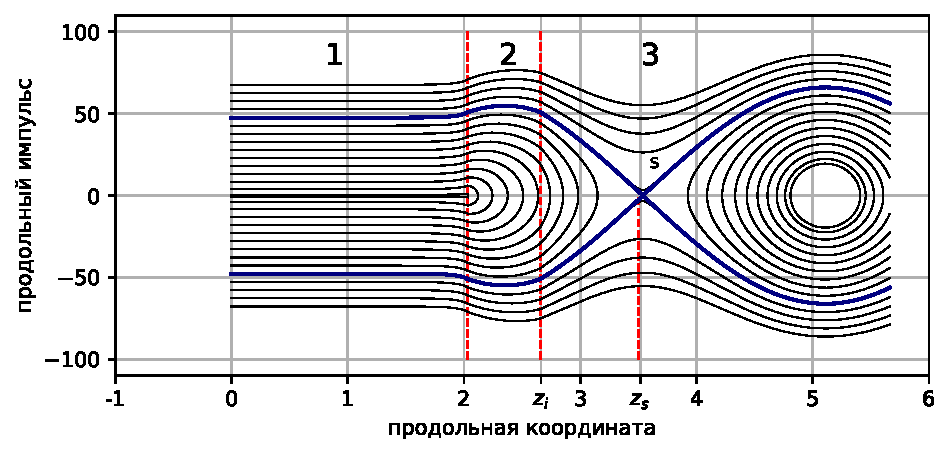
\includegraphics[width=\linewidth]{pic/fas_port.pdf}	
                    %\hfill
                    \end{minipage}
                   % \begin{minipage}{0.32\linewidth}
                    %        \centering
                     %    \includegraphics[width=\linewidth]{}
                    %\end{minipage}
                    %\begin{minipage}{0.32\linewidth}
                     %       \centering
                    %\vspace{-15pt}
                     %       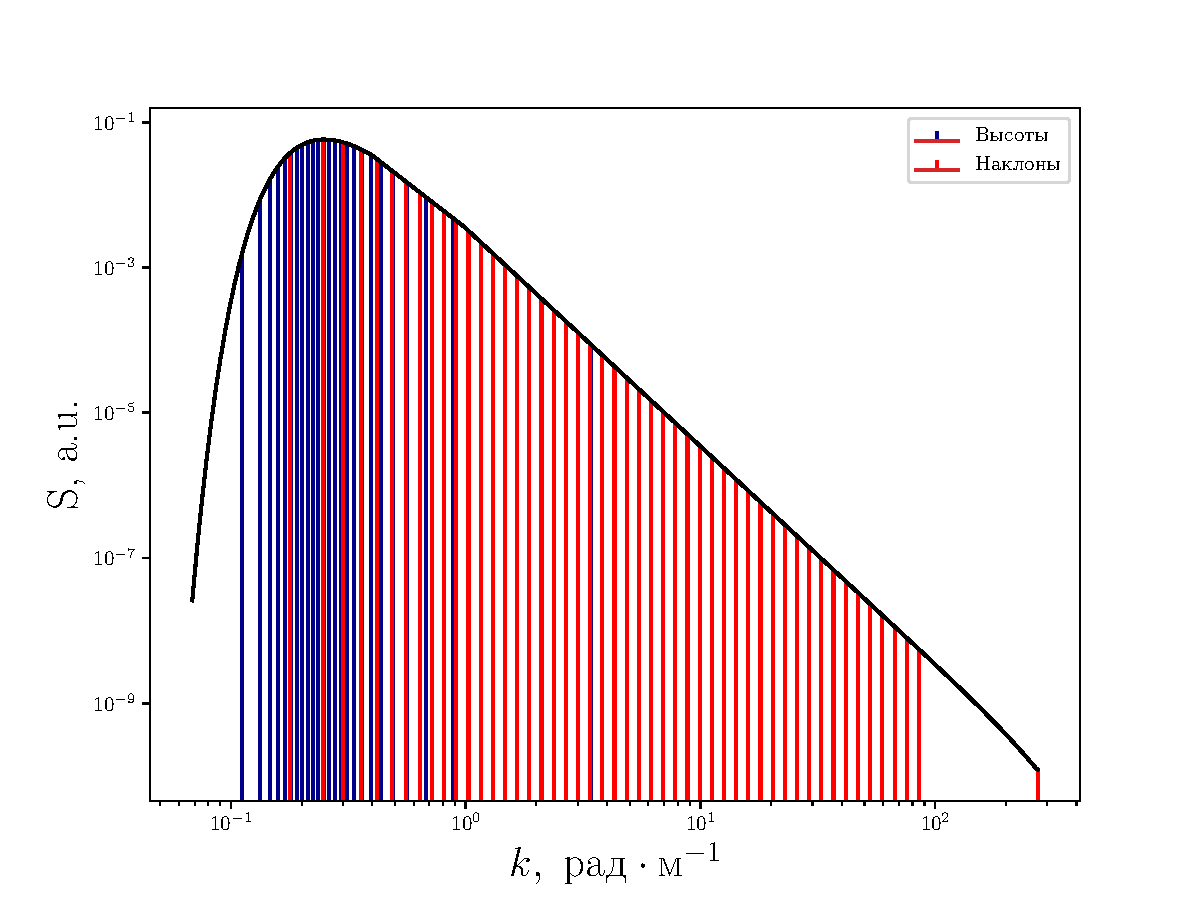
\includegraphics[width=\linewidth]{nodes}
                    %\end{minipage}

                    %\begin{minipage}{0.38\linewidth}
                     %       \centering
                      %      \includegraphics[width=\linewidth]{pic/1.jpg}
                       %     $n_0=10$
                    %\hfill
                    %\end{minipage}

                    %\begin{minipage}{0.38\linewidth}
                     %       \centering
                       
                       %     \includegraphics[width=\linewidth]{pic/2.jpg}
                        %    $n_0=20$
                    %\hfill
                    %\end{minipage}
                    %\begin{minipage}{0.38\linewidth}
                     %       \centering
                           
                           % \includegraphics[width=\linewidth]{pic/3.jpg}
                            %$n_0=30$
                    %\hfill
                    %\end{minipage}

                    %\caption{Располо
                  
                   
                    %\caption{Располо
                    %\caption{Располо
                    %\caption{Расположении узлов по методу <<отбеливания>> спектра  для (a) наклонов и (b) высот соответственно. $U=10 \frac{\text{м}}{c}$, $N=25$; (c) суперпозиция 
                    %метода <<отбеливания>> для высот и наклонов}
                    %\label{fig:splits}	
                    \label{fig:spec}
            \caption{Фазовый портрет пробного электрона при $n_0=15, a_{\text{пад}}=33$}	
                \end{figure}

                \begin{figure}[H]
                    \begin{minipage}{0.6\linewidth}

                            \centering
                            \includegraphics[width=\linewidth]{}	
                    %\hfill
                    \end{minipage}

                    \label{fig:spec}
            \caption{Зависимость критического импульса от коцентрации и скорости электронов}	
                \end{figure}
                %\begin{figure}[h]
                 %   \centering
                  %  \begin{minipage}{0.49\linewidth}
%                           \centering
  %                          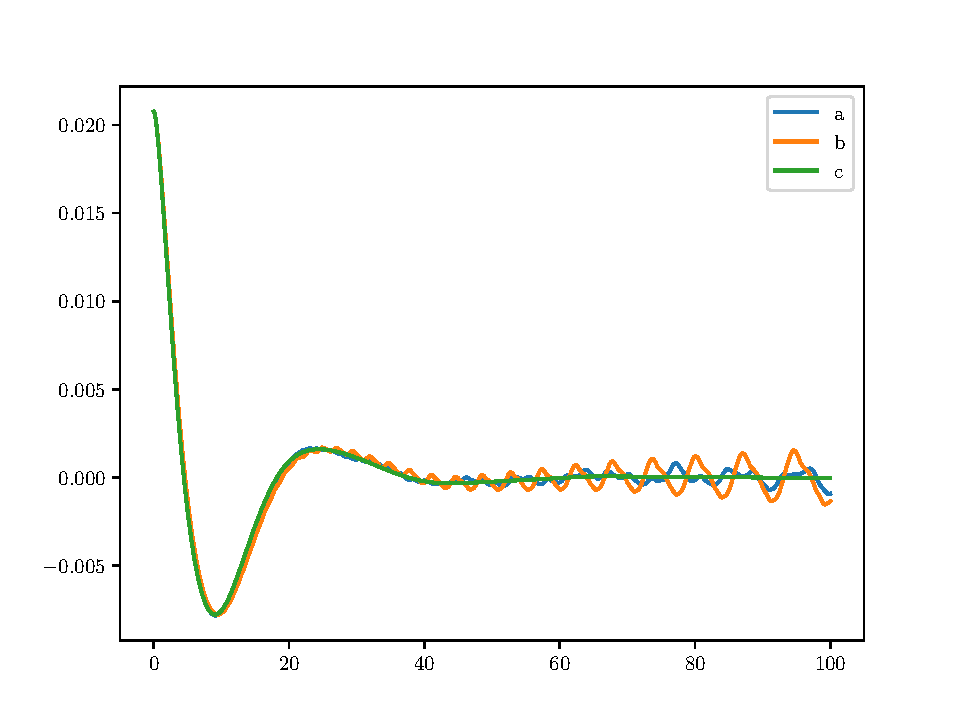
\includegraphics[width=\linewidth]{fig/corr1}

 %                           (a)
  %                  \end{minipage}
   %                 \begin{minipage}{0.49\linewidth}
    %                        \centering
     %                      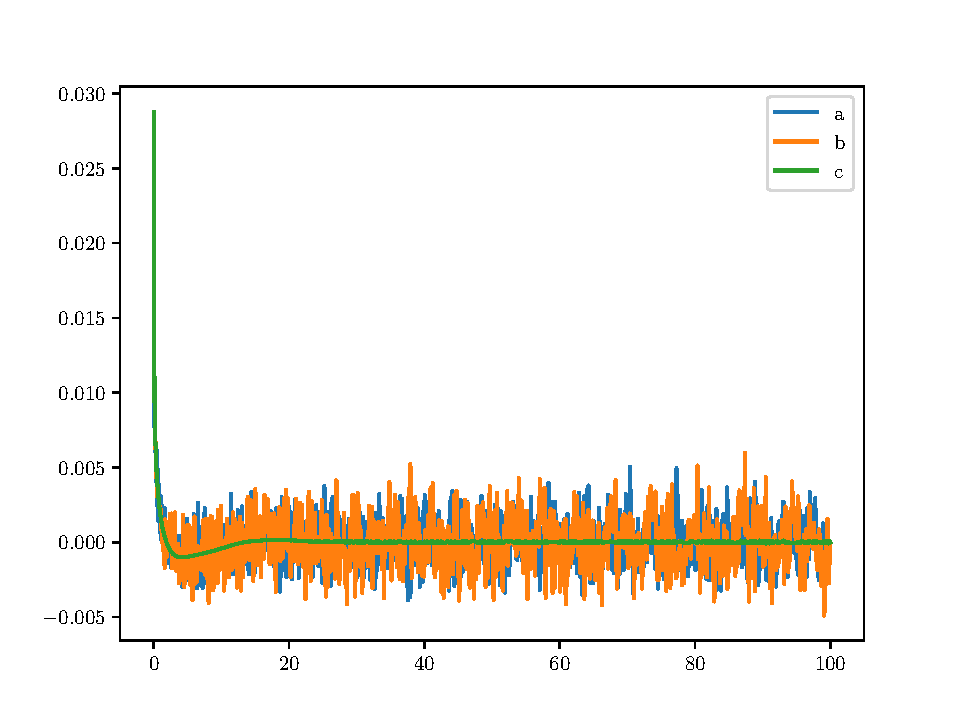
\includegraphics[width=\linewidth]{fig/corr2}

                  %          (b)
                 %   \end{minipage}
                    %\caption{Корреляционные функции высот и уклонов  при различных расположениях гармоник. $U=5\frac{\text{м}}{\text{с}},~ N = 128$; 
                    %(a) расположение по методу <<отбеливания>> спектра, 
                    %(b) логарифмическое расположение;
                    %(c) теоретическая корреляционная функция }
                    %\label{fig:}
                %\end{figure}
        \end{block}
        \begin{block}{Заключение}
            %\small
 			\begin{enumerate}
            \item в работе исследована система и развит метод построения лазерно-плазменных структур при ускорении ионов радиационным давлением
           \item построены решения
       	\item разработан алгоритм построения фазового портрета и нахождения критического импульса для данной системы
       	\item полученные значения критического импульса велики, что говорит об устойчивости данной структуры относительно продольной температуры
 			\end{enumerate}
            %
           %предложенный в \cite{CWM}, 

 
        \end{block}
        \begin{block}{Литература}
            \footnotesize
            \begin{thebibliography}{}
                \bibitem{cite1} \textit{А.В. Коржиманов. В.И. Еремин, А.В. Ким, М.Р. Тушенцов}
                О взаимодействии релятивистски сильных электромагнитных волн со слоем закритической плазмы // ЖЭТФ, 2007. Т.132, вып.4(10).  C. 771.

                \bibitem{}    \textit{Д.А.Войтович, А.В Коржиманов} Стационарные лазерно-плазменные структуры при ускорении ионов радиационным давлением в режиме «плуга» // Труды XXIII научной конференции по радиофизике, посвященной 100-летию со дня рождения Н.А.Железнова Национальный исследовательский Нижегородский государственный университет им. Н.И. Лобачевского. Нижний Новгород, 2019.C. 332-333.
    
    			\bibitem{} \textit{E. Siminos, M. Grech,S. Skupin,T. Schlegel,and V. T. Tikhonchuk} Effect of electron heating on self-induced transparency in relativistic-intensitylaser-plasma interactions //PHYSICAL REVIEW E 86, 056404, 2012.
    			\bibitem{} \textit {Andrea Macchi, Marco Borghesi, Matteo Passoni} Ion acceleration by superintense laser-plasma interaction //RMP, 2013. Vol. 85. C.773.

                
            \end{thebibliography}
        \end{block}
      \end{column}
    \end{columns}
  \end{frame}

\end{document}
